\section{Lecture 3: Matter as a wave}

\subsection{Everything is a wave (in Quantum Mechanics)}

Whether we analyze something as a particle versus wave is really a question of system size versus wavelength.
For example, for the de Broglie wavelength (for an electron orbital), angular momentum is quantized, so:
\begin{align*}
    \lambda_{dB} &= \frac{h}{p} ~ nm
\end{align*}
versus the size of an atom is on the order of an angstrom, much smaller.

However for a human
\begin{align*}
    \lambda_{dB} &= 10^{-36} m
\end{align*}
versus the size of a human is on the order of a meter.

Waves can interfere. Suppose you have a light wavefront like this.

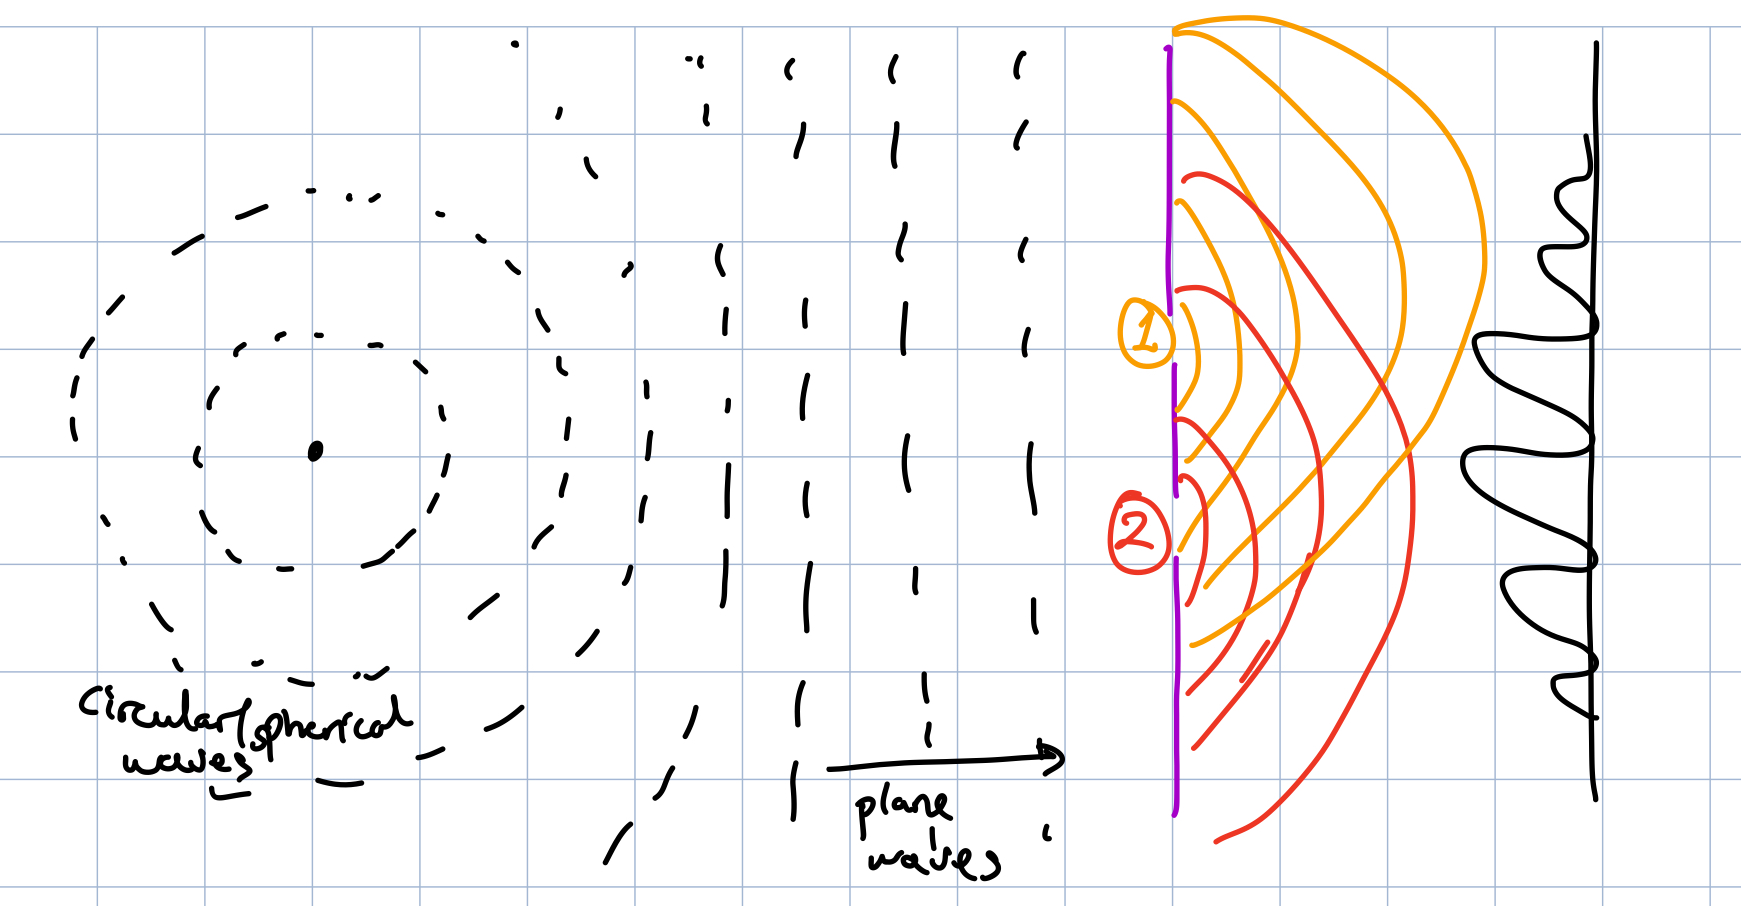
\includegraphics[width=300px]{wavefronts.jpeg}

We will focus on the case of a plane wave since the mathematics is simpler. We use complex exponentials to represent the waves. The electric field is:
\[ \mathbf{E} = \mathbf{E}_0  e^{i(\mbf{k} \cdot \mbf{r} - \omega t + \phi)} \]
The amplitude is a vector (direction for which direction the wave wiggles in). The phase $\delta = (\mbf{k} \cdot \mbf{r} - \omega t + \phi)$ can be decomposed.
$\mbf{k}$ is the spatial frequency and $\omega$ is the time frequency. Then $\phi$ is the wave phase at $(\mbf{r}, t) = (\mbf{0}, 0)$.
We can get the total electric field by using simple superposition principle.
\begin{align*}
    \mbf{E}_{tot} &= \mbf{E}_1 + \mbf{E}_2 \\
    &= \mbf{E}_{01} e^{i \delta_1} + \mbf{E}_{02} e^{i \delta_2}
\end{align*}
In practice, we measure a scalar quantity intensity $I$,
\begin{align*}
    I \sim |\mbf{E}|^2 &= \mbf{E} \cdot \mbf{E}^* \\
    &= E_{01}^2 + E_{02}^2 + \mbf{E}_{01} \cdot \mbf{E}_{02} \qty(e^{i (\delta_2 - \delta_1)} + e^{-i(\delta_2 - \delta_1)}) \\
    &= E_{01}^2 + E_{02}^2 + 2 \mbf{E}_{01} \cdot \mbf{E}_{02} \cos(\delta_2 - \delta_1)
\end{align*}
However, they did the same experiment with electrons and got the same result. Matter must itself be a wave!

\subsection{The Wavefunction}
Now we want a wave description of matter. The $\mbf{E}$ is not sufficient for these purposes. We will use $\Psi$ as this "wavefunction." Some weird properties
of $\Psi$ is:
\begin{itemize}
    \item $\Psi$ is a wave amplitude.
    \item It is not physical and cannot directly be measured.
    \item This function contains all the information about your system.
\end{itemize}
Max Born in 1926 gave the following interpretation to $\Psi$.
\begin{theorem}[Born Rule]
    If the wavefunction of a system is $|\Psi|^2$ is a probability (spatial) density to find the "particle" around $\mbf{r}, t$.
\end{theorem}
With repeated measurements, the long-time probability for finding the particle within a cube $\dd{\mbf{r}}$ becomes:
\[ P(\mbf{r}, t) \dd{\mbf{r}} = |\Psi(\mbf{r}, t)|^2 \dd{\mbf{r}} \]
\begin{theorem}[Superposition]
    If $\Psi_1, \Psi_2$ are allowed waves (solutions), then:
    \[ \Psi = c_1 \Psi_1 + c_2 \Psi_2 \]
    is also a viable solution, $\{c_1, c_2\} \in \mathbb{C}$.
\end{theorem}
Think about your favorite particle. It looks something like this:

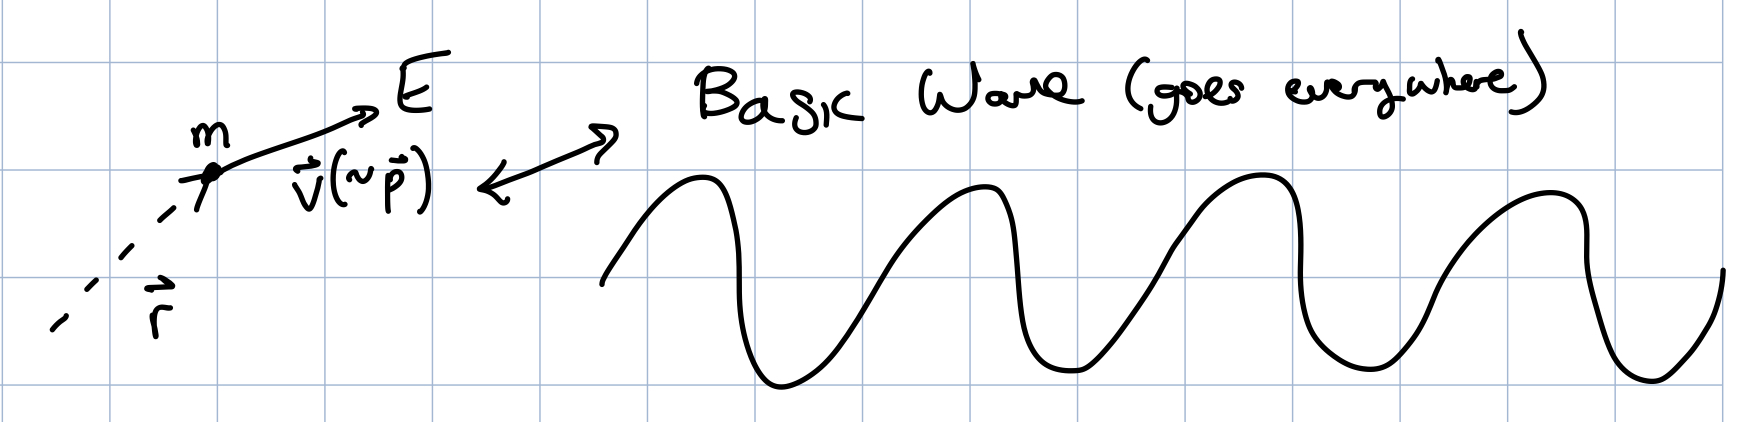
\includegraphics[width=400px]{basic_wave.jpeg}

Unfortunately this basic wave spills everywhere in space. It is a good approximation for certain scales (say the double-slit setting), but not perfect. This is how our physics translates: 
\begin{align*}
    E &= hf = \hbar \omega \\
    p &= \frac{h}{\lambda} = \hbar k
\end{align*}
where $\hbar = \frac{h}{2\pi}$ and $k = \frac{2\pi}{\lambda}$.

Consider a 1-D particle with some $x$ direction momentum $p_x$.
\begin{align*}
    \Psi &= A e^{i(k x - \omega(k) t)} \\
    \Psi &= Ae^{i(p_x x - E(p_x) t)} \\
\end{align*}
Thus simply by derivative rules, the "momentum operator" $p_x$ is:
\[ - i \hbar \partialderivative{}{x} \Psi = p_x \Psi \]
\[ i \hbar \partialderivative{}{t} \Psi = E \Psi \]
In 3-D, we have (using dot products):
\[ \mbf{p} = \hbar \mbf{k} \]
which means that the operator looks like:
\[ - i \hbar \nabla \Psi = \mbf{p} \Psi\]
